%!TEX program=xelatex
\documentclass[a4paper]{article}
\usepackage{ctex}
\usepackage{geometry}
\usepackage{multirow}
\usepackage{tabularx}
\usepackage{float}
\usepackage{graphicx}
\usepackage{diagbox}

\geometry{left=3.0cm,right=3.0cm,top=3.5cm,bottom=3.5cm}

\title{逸出功的测量}
\author{2017011341, 陈旭}
\date{2019 年 3 月}

\begin{document}

\maketitle

\section{实验目的}

\begin{itemize}
	\item 用里查孙直线法测定阴极材料(钨)的电子逸出功;
	\item 了解热电子发射的规律;
	\item 掌握逸出功的测量方法。
\end{itemize}

\section{实验原理}

\par 由于金属与真空之间有位能壁垒$W_a$,因此电子要从金属中逸出,必须具有大于$W_a$的动能。$W_0=W_a-W_i$即为逸出功。

\par 关于热电子发射的里查孙——德西曼公式
$$J_e=2(1-R_e)A_1T^2e^{-(W_a-W_i)/kT}$$
\par 其中 $J_e$ 为单位面积的发射电流;$W_a-W_i=e_0 \phi$ 为该金属的逸出功,单位常用电子伏特表示;$phi$称为逸出电位;$A_1$为普适常数,$A_1=60.09A/(cm\cdot K)^2$;$R_e$为金属表面对发射电子的反射系数。

\par 若令$2(1-R_e)A_1=A$,则有$AT^2e^{-e_0\phi/kT}$;可得发射电流的公式:
$$I_e=AST^2e^{-e_0\phi/KT}$$
\par 其中$S$为阴极金属的有效发射面积。

\section{数据处理原理}

\subsection{$A$与$S$的处理}

\par $A$与$S$这两个量在实际实验中难以测量,甚至无法测量。因此需对上述公式作适当处理,使$\lg(\frac{I_e}{T^2})$与$\frac{1}{T}$成线性关系,便可以由直线的斜率求得$\phi$的大小,此方法即查孙直线法。

\par 经过处理后的公式为:
$$\lg(\frac{I_e}{T^2})=\lg(AS)-5.039\times 10^3\frac{\phi}{T}$$

\subsection{发射电流$I_e$的测量}

\par 一般情况下,外加电压$U_a>>U'_a$,所以有:
$$\lg I'_e=\lg I_e+\frac{4.39}{2.303T}\cdot\frac{1}{\sqrt{r_1\ln(r_2/r_1)}}\sqrt{U_a}$$
\par 由此可见,在阴极温度一定的情况下,$\lg I'_e$与$\sqrt{U_a}$成线性关系。所以可以画出在不同阴极温度下的$\lg I'_e$与$\sqrt{U_a}$的关系曲线,并将其外推至$\sqrt{U_a}=0$处,此时$\lg I'_e$即为$\lg I_e$,由此可以定出所需要的$I_e$值。

\subsection{温度$T$的测量}

\par 通过测量阴极加热电流来确定阴极温度。对于纯钨丝,一定的比加热电流$I_1$与阴极温度的关系已有前人精确地测算并列成表。

\par 根据公式$I_1=I_f/(d_K)^{3/2}$可以由阴极电流的大小得出比加热电流的大小,从而查表得出对应的温度$T$。其中$I_f$为阴极加热电流,$d_K$为阴极钨丝直径。

\section{实验任务}

\begin{itemize}
	\item 根据二极管的结构和测量的原理以及电压测量电路和加速电源线路设计好使用而完整的实验线路图。
	\item 根据教师审查过的设计线路图接线。
	\item 在一定灯丝温度(对应于某一灯丝电流)下,测定加速电压$U_a$和阳极电流$I'_e$的关系。$U_a$从$25V$开始逐步增加,测$6\sim7$个点。
	\item 灯丝电流从$0.50A$开始,每隔$0.04A$作一次上述测定,最大电流取$0.70A$。调节时灯丝电流不宜超过$0.75A$,以延长灯丝寿命。
	\item 用直线拟合法处理数据:求出$\phi$值和逸出功$e_0\phi$的值。
	\item 作$\lg I'_e-\sqrt{U_a}$曲线和$\lg(\frac{I_e}{T^2})-\frac{1}{T}$曲线,根据图像求出$\phi$,从而得到逸出功$e_0\phi$的值。
\end{itemize}

\section{数据记录与处理}

\begin{table}[H]
	\centering
	\resizebox{\textwidth}{20mm}{
		\begin{tabular}{|c|c|c|c|c|c|c|c|c|c|c|c|c|}
			\hline
			\multicolumn{2}{|c|}{\multirow{2}{*}{\diagbox{$I_f(A)\ T(K)$}{$U_a(V)$}}} & 36.00  & 49.00  & 64.00  & 81.00  & 100.00 & 121.00 & 144.00 & \multirow{2}{*}{$\frac{1}{T} (10^{-4})$} & \multirow{2}{*}{$I_e$} & \multirow{2}{*}{$\lg(\frac{I_e}{T^2})$} & \multirow{2}{*}{$r^2$} \\ \cline{3-9}
			\multicolumn{2}{|c|}{}                     & 6.00   & 7.00   & 8.00   & 9.00   & 10.00  & 11.00  & 12.00  &                                               &                     &                                             &                    \\ \hline
			0.50                 & 1726                & 4.10   & 4.20   & 4.30   & 4.40   & 4.49   & 4.60   & 4.70   & 5.7937                                   & 0.0013              & -9.3513                                & 0.9996             \\ \hline
			0.54                 & 1795                & 16.06  & 16.40  & 16.75  & 17.09  & 17.42  & 17.77  & 18.11  & 5.5710                                   & 0.0053              & -8.7854                                & 0.9996             \\ \hline
			0.58                 & 1862                & 48.31  & 49.35  & 50.38  & 51.40  & 52.39  & 53.42  & 54.46  & 5.3706                                   & 0.0159              & -8.3386                                & 0.9996             \\ \hline
			0.62                 & 1929                & 131.00 & 133.63 & 136.30 & 138.68 & 141.08 & 143.54 & 146.02 & 5.1840                                   & 0.0436              & -7.9308                                & 0.9989             \\ \hline
			0.66                 & 1995                & 370.7  & 377.7  & 384.5  & 391.1  & 397.7  & 404.6  & 411.6  & 5.0125                                   & 0.1239              & -7.5070                                & 0.9997             \\ \hline
			0.70                 & 2058                & 848.7  & 864.7  & 880.3  & 895.8  & 910.4  & 925.9  & 941.5  & 4.8591                                   & 0.2839              & -7.1738                                & 0.9995             \\ \hline
		\end{tabular}}
	\caption{逸出功的测量实验数据记录}
\end{table}

\begin{figure}[H]
	\centering
	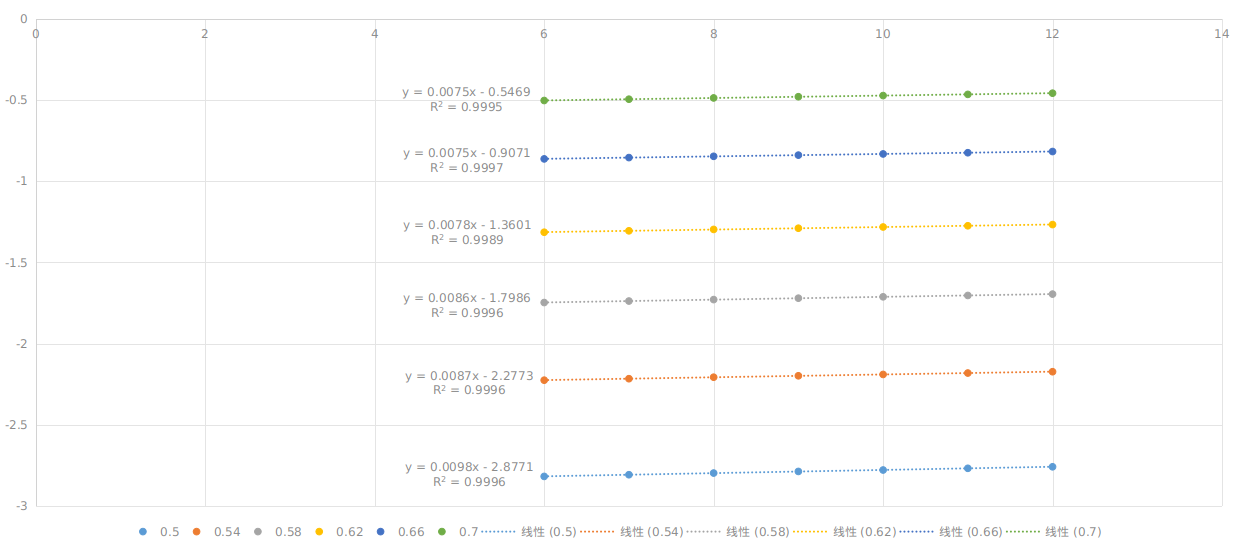
\includegraphics[width=0.9\linewidth]{figures/f1}
    \caption{$\lg(I_e^\prime)-\sqrt{U_a}$ 直线拟合结果}
\end{figure}

\begin{figure}[H]
	\centering
	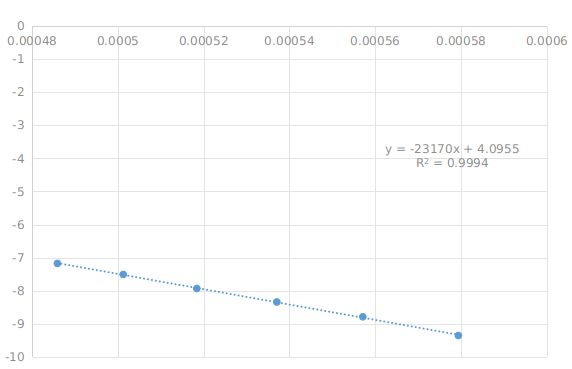
\includegraphics[width=0.9\linewidth]{figures/f2}
    \caption{$\lg(\frac{I_e}{T^2})-\frac{1}{T}$ 直线拟合结果}
\end{figure}

\par 由拟合结果可得:

$$
\begin{array}{rcccl}
	\Phi&=&\frac{-23216}{-5039}&\approx&4.598\\
	W_0&=&e_0\times \Phi&\approx&7.357\times 10^{-19}\ J
\end{array}
$$

\par 计算不确定度:

$$
\begin{array}{cl}
	&\frac{D_f}{f}=\frac{D_k}{k}=\sqrt{\frac{\frac{1}{r^2}-1}{n-2}}\approx 0.01225\\
	&D_f=\frac{D_f}{f}\times f\approx 0.056\ V\\
	&D_W=\frac{D_f}{f}\times W_o\approx 0.090\ J
\end{array}
$$

\par 所以:

$$
\begin{array}{rcl}
	f&=&(4.598\pm 0.056)\ V\\
	W_0&=&(7.357\pm 0.090)\times 10^{-19}\ J
\end{array}
$$

\section{思考题}

\subsection{$I_f$ 系统误差修正的必要性}

\par 不需要,外部两个 $18k\Omega$ 电阻串联,阻值远大于灯丝电阻,流经该支路的电流远小于电流表仪器误差,可忽略不计。

\subsection{$U_a$ 系统误差修正的必要性}

\par 不需要,电路中 $R_4$ 远大于 $R_5$,因此 $U_a$ 的系统误差将远小于恒压源的输出电压,可忽略不计。

\subsection{$U_e^\prime$ 是否必须化为 $I_e^\prime$ 再进行数据处理?}

\par 不需要,$U_e^\prime$ 与 $I_e^\prime$ 成正比例关系,取对数后只相差一个常数,在拟合时只影响截距,而我们只需要拟合结果的斜率。

\subsection{C 点是否为灯丝中点电位等效点?}

\par 是,C 点位于两个 $18k\Omega$ 的电阻中间,简单计算可得其电位等于灯丝中点电位。

\section{实验体会}

\par 通过里查孙直线法,我发现在一些问题中有的量是难以测量的,但是可以先从数学上对相关公式进行化简,从而找到更容易的实验方法。

\newpage

\section{附录}

\begin{figure}[H]
	\centering
	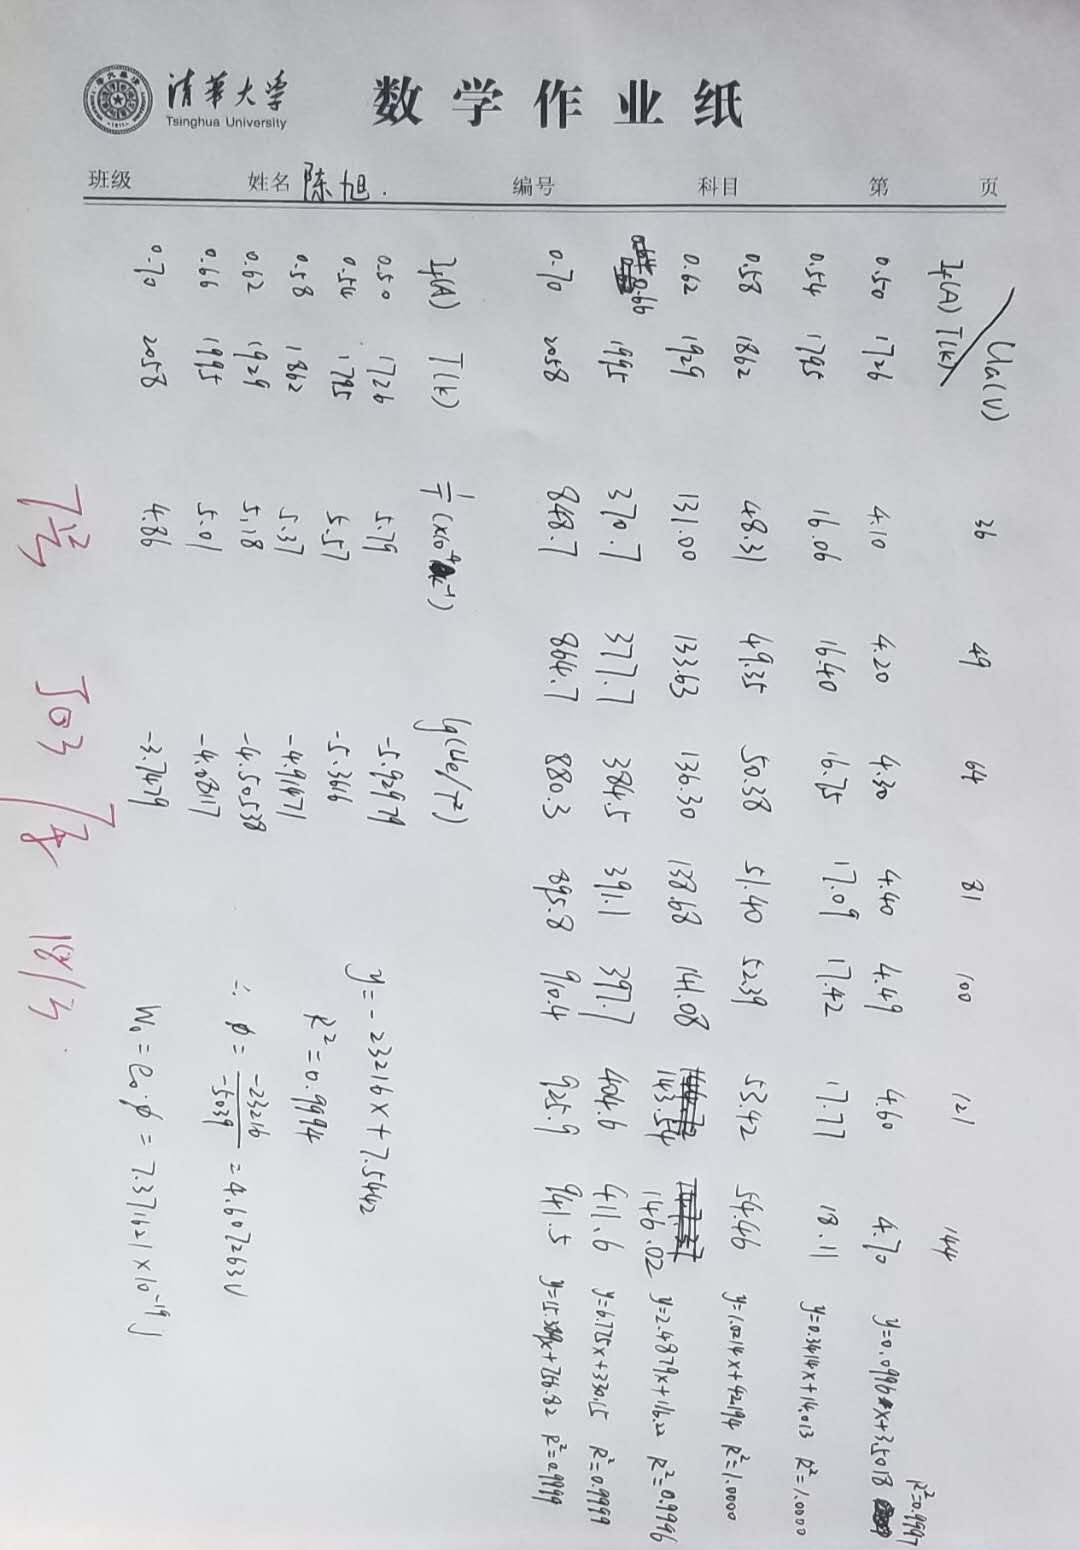
\includegraphics[width=0.9\linewidth]{figures/f3}
    \caption{实验原始数据(图中计算结果有误,仅原始数据可供参考)}
\end{figure}

\end{document}